\documentclass[aspectratio=43,unicode,10pt]{beamer}
\usetheme{ttipresentation}

\usepackage{luatexja}
\usepackage{luatexja-fontspec}
\usepackage{graphicx}
\usepackage{multicol}

\setmainjfont{ipagp.otf}
\beamertemplatenavigationsymbolsempty

\newcommand{\itemtitle}[1]{\textbf{#1}\\}
\newcommand{\fire}[1]{\textcolor{red}{\textbf{#1}}}
%\newcommand{\freeze}[1]{\textcolor{blue}{\textbf{#1}}}
\newcommand{\then}{\textcolor{ttiblue}{\textbf{⇒}}\hspace{1ex}}
\newcommand{\good}{\textcolor{orange}{\textbf{◎}}\hspace{1ex}}
\newcommand{\arrow}{\textcolor{ttiblue}{\textbf{→}}\hspace{1ex}}
\abovedisplayskip=0pt
\belowdisplayskip=0pt


\title{文書・文間及びカテゴリ間の関係を\\考慮したレーティング予測}
\institute{知能数理研究室}
\author{12056 外山 洋太}
\date{\today}



\begin{document}

\begin{frame}{パラグラフベクトル}{}
\end{frame}

\begin{frame}{文ベクトルの重み付け平均の式}{}
  \begin{gather*}
    L = \frac{1}{T} \sum^{T}_{t = k} \log p(w_t | w_{t-k}, ..., w_{t-1}),
      \label{eq:ParagraphVector} \\
    p(w_t | w_{t-k}, ..., w_{t-1}) = \frac{e^{y_{w_t}}}{\sum_i e^{y_i}},
      \nonumber \\
    y = b + Uh(w_{t-k}, ..., w_{t-1}, d; W, D) \nonumber
  \end{gather*}
  \begin{itemize}
    \footnotesize
    \item $d$:文章
    \item $w_i$:単語
    \item $W$:全ての単語の分散表現を表す行列
    \item $D$:全ての文章の分散表現を表す行列
    \item $k$:ウィンドウサイズ
    \item $T$:現在の文章に含まれる単語数
    \item ウィンドウ:ある単語の周辺を表す区間
    \item $p$:softmax関数により正規化された、
          文脈から現在の単語が導かれることの尤度
    %\item $y$:現在の単語とウィンドウ内の単語及び現在の文章から導出
    \item $h(w_{t-k}, ..., w_{t-1}, d; W, D)$:
          引数となるベクトルを結合したベクトルを返す関数
  \end{itemize}
\end{frame}

\begin{frame}{文間・カテゴリ間の関係}{}
  \begin{columns}[t]
    \begin{column}{0.6\textwidth}
      \begin{block}{文間の関係}
        「とても良かった」の文が
        \begin{itemize}
          \item 食事に関する文の直後に存在 \\
                \then 食事\good
          \item 部屋に関する文の直後に存在 \\
                \then 部屋\good
        \end{itemize}
        \begin{figure}
          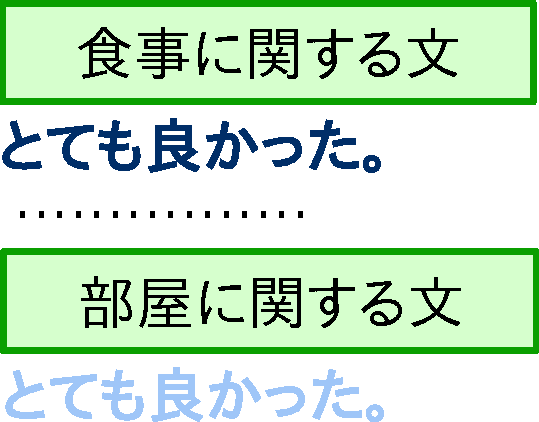
\includegraphics[width=0.6\linewidth]
                          {fig/global_relations_among_sentences_v2.pdf}
        \end{figure}
      \end{block}
    \end{column}
    \begin{column}{0.4\textwidth}
      \begin{block}{カテゴリ間の関係}
        \begin{itemize}
          \item 他のカテゴリ\good \\
                \then 「総合」カテゴリ\good
        \end{itemize}
        \begin{figure}
          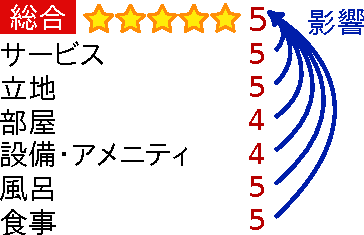
\includegraphics[width=\linewidth]
                          {fig/relations_among_rating_categories.pdf}
        \end{figure}
      \end{block}
    \end{column}
  \end{columns}
\end{frame}

\begin{frame}{関連研究}{}
  \begin{block}{隠れ状態を用いたホテルレビューのレーティング予測
                \footnote[frame]{
    藤谷宣典ら,
    隠れ状態を用いたホテルレビューのレーティング予測.
    言語処理学会第21回年次大会, 2015.
  }\\(従来手法)}
    \begin{itemize}
      \item 文毎のレーティングからレビュー全体のレーティングを予測
      \item カテゴリ間の繋がりを\fire{手調整で変化}させて考慮
    \end{itemize}
    \begin{figure}
      \vspace{-1em} % HACK
      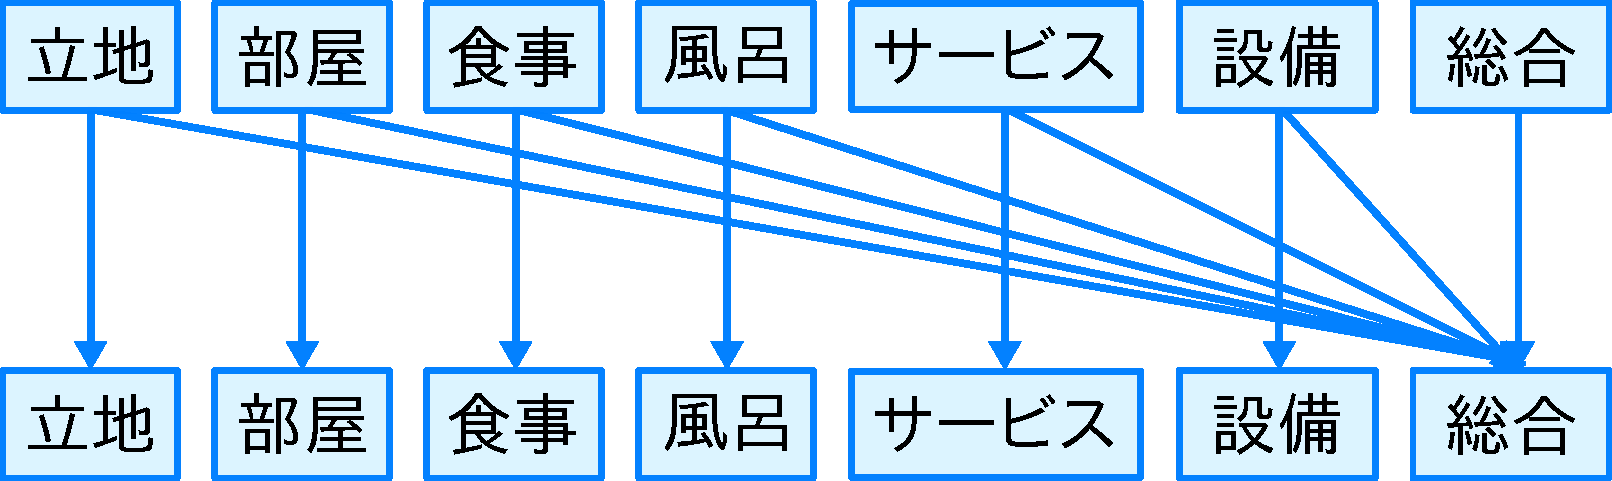
\includegraphics[width=0.5\linewidth]
                      {fig/fujitani_miml_relations_among_rating_categories.pdf}
      \vspace{-1em} % HACK
    \end{figure}
  \end{block}
  \begin{block}{パラグラフベクトル
                \footnote[frame]{
    Quoc Le et al.,
    Distributed representations of sentences and documents.
    ICML 2014, 2014.
  }}
    \begin{itemize}
      \item 文や文書を実数ベクトルに変換する手法
      \item \fire{レーティング予測において優れた性能}
    \end{itemize}
  \end{block}
  %\begin{block}{ニューラルネットワーク}
  %  \begin{itemize}
  %    %\item 神経回路を模した機械学習手法
  %    %\item 分類問題に適用可能
  %    \item \fire{入力間・出力間の複雑な関係}を考慮
  %  \end{itemize}
  %\end{block}
\end{frame}

\begin{frame}{提案手法}{}
  \begin{itemize}
    \item 文書・文間及びカテゴリ間の関係を自動で考慮した\\レーティング予測
    \item パラグラフベクトルと\fire{入出力間の複雑な関係を考慮}できる \\
          ニューラルネットワークを利用
  \end{itemize}
  %\begin{enumerate}
  %  \item パラグラフベクトルにより各レビューとその中の文のベクトルを生成
  %  \item 文ベクトルをレビュー毎に圧縮
  %  \item ニューラルネットワークによりレーティングを予測
  %\end{enumerate}
  \begin{figure}
    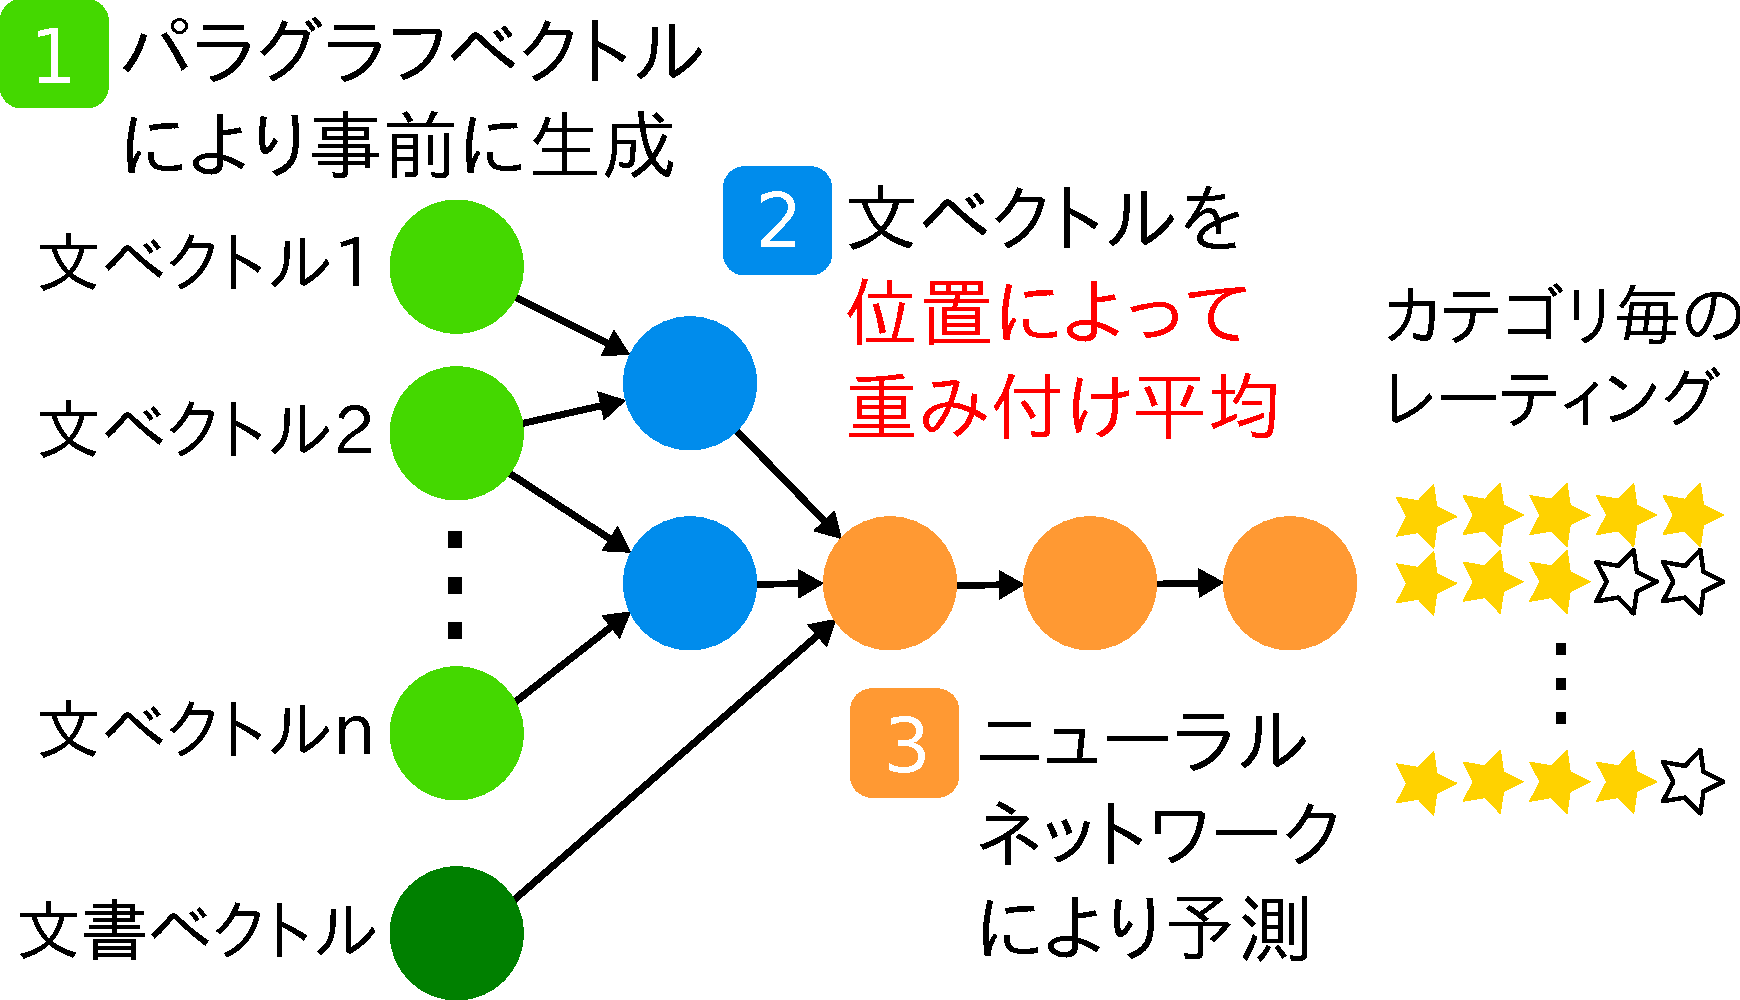
\includegraphics[width=0.8\linewidth]
                    {fig/model_with_detailed_processes.pdf}
  \end{figure}
\end{frame}

\begin{frame}{実験}{}
  \begin{block}{実験設定}
    \begin{itemize}
      \item 7カテゴリにおける0〜5点のレーティング予測の正答率を測定
      \item データセット:楽天トラベルにおけるレビュー約330,000件
    \end{itemize}
  \end{block}
  \begin{block}{結果}
    \begin{columns}[onlytextwidth,t]
      \begin{column}{0.6\linewidth}
        \begin{itemize}
          \item 提案手法が従来手法より\fire{高い正答率}を示した
          %\item \fire{文の並び}が予測のために重要
          %\item 文書ベクトルと文ベクトルを同時に用いることが有効
        \end{itemize}
      \end{column}
      \begin{column}{0.4\linewidth}
        \begin{table}
          \centering
          \begin{tabular}{l | r}
            手法 & 正答率 {[}\%{]} \\
            \hline
            従来手法 & 48.32 \\
            提案手法 & \fire{50.30} \\
          \end{tabular}
        \end{table}
      \end{column}
    \end{columns}
  \end{block}
\end{frame}

\end{document}
